\documentclass[xcolor=dvipsnames,beamer]{beamer} %handout,notes=show

\usepackage{textcomp}
\usepackage[utf8]{inputenc}
% \usepackage{default}
\usepackage{graphicx}
%  \usepackage[pdftex]{hyperref}
\usepackage{url}
\usepackage{amsmath}

% frames have to be fragile
\newif\ifnotes
% \notestrue

%\notestrue


\ifnotes
%\setbeamertemplate{note page}[plain]
\setbeamertemplate{note page}[compress]
\setbeamerfont{note page}{size=\large}
\setbeameroption{show only notes}
%\setbeameroption{show notes}
\usepackage{pgfpages}
\pgfpagesuselayout{2 on 1}[a4paper,border shrink=5mm]%
\else
%\setbeameroption{hide notes}
\fi
%\notesfalse



% nastaveni TypeWriter
%\usepackage{courier}
%\usepackage{lmodern}
%\renewcommand*\ttdefault{txtt}
\DeclareFontShape{OT1}{cmtt}{bx}{n}{<5><6><7><8><9><10><10.95><12><14.4><17.28><20.74><24.88>cmttb10}{}


% \usepackage{verbatim}
\usepackage[absolute,overlay]{textpos}

\usepackage{listings}
% \usepackage{courier}
\definecolor{grey}{RGB}{70,70,70}
\definecolor{green}{RGB}{0,255,0}
\definecolor{red}{RGB}{202,53,53}
\definecolor{lightGrey}{RGB}{250,250,250}
\definecolor{darkGrey}{RGB}{50,50,50}


\usepackage{color}
\definecolor{lightgray}{rgb}{.9,.9,.9}
\definecolor{darkgray}{rgb}{.4,.4,.4}
\definecolor{purple}{rgb}{0.65, 0.12, 0.82}


% \usetheme{Warsaw}
% \usetheme{Madrid}
\usetheme{Szeged}
% \useoutertheme{infolines}
% \usecolortheme[named=MidnightBlue]{structure}
\usecolortheme[named=PineGreen]{structure}
% \setbeamertemplate{navigation symbols}{}




\title[The Mountains and the Ants]
{Perspectives on FOSS GIS/RS \\Research \& Teaching in SSEA}
%\subtitle{SVO\v{C}}
%\pdforstring{}{}
\author[Yann Chemin]
{Yann Chemin}

\institute[U. of Moratuwa - IWMI]
{International Water Management Institute\\ University of Moratuwa
\vspace{20pt}
% 
\includegraphics[width=1cm]{iwmi}
}
\date{June 12, 2013}


%\AtBeginSection[]{\begin{frame}\frametitle{Obsah}%
%\tableofcontents[currentsection ]\end{frame}}
%\AtBeginSubsection[]
%{
%  \begin{frame}<beamer>
%  \frametitle{Obsah}
%  \tableofcontents[currentsection,currentsubsection]
%  \end{frame}
%}

\setbeamercovered{transparent}

\hypersetup{%
	pdfauthor={Yann Chemin},%
	pdfsubject={Presentation},%
    pdfkeywords={OSGEO, IWMI, Moratuwa}
}

\usepackage{listings}
\lstdefinestyle{C++}{%
  % language
  language=C++, % [ANSI]C++, GNU, ISO, Visual
  basicstyle=\ttfamily\small,
  commentstyle=\itshape,
  keywordstyle=\bfseries, % needs another \ttdefault
  showstringspaces=false,
  stringstyle=,
  identifierstyle=,
  % working with latex
  escapeinside={//lst}{\^^M}  
}

\lstset{%
%  frame=trBL,
%  backgroundcolor=\color{},
  linewidth=\textwidth,
  % working with latex
  gobble=2,
  % float
  nolol=false,
  numberbychapter=true,
  captionpos=t,% tb
  % breaking lines
  breaklines=true,
  breakatwhitespace=true,
  breakindent=10em,
  breakautoindent=true,
  prebreak={},
  postbreak={},
  %document default style
    basicstyle=\ttfamily
}


%\lstlistlistingname % The header name for the list of listings.
%\lstlistingname % The caption label for listings.

\lstnewenvironment{cmdline}[1][]
{\lstset{
  style=C++,
  #1}}
{}

\lstnewenvironment{scpp}[1][]
{\lstset{
  style=C++,
  #1}}
{}

\lstnewenvironment{ncpp}[1][]
{\lstset{
  style=C++,
  numbers=left, 
  numberstyle=\scriptsize, 
  stepnumber=1,
  numbersep=5pt,
  #1}}
{}

\lstnewenvironment{fcpp}[1][]
{\lstset{
  style=C++,
  float,
   % line numbers
  numbers=left, 
  numberstyle=\scriptsize, 
  stepnumber=1,
  numbersep=5pt,
  #1}}
{}


\lstnewenvironment{lcpp}[1][]
{\lstset{%
style=C++,
numbers=left, 
numberstyle=\scriptsize, 
stepnumber=1,
numbersep=5pt,
xleftmargin=12pt,
breakautoindent=false,
breaklines=false,%
#1}}{}

\lstnewenvironment{smallcpp}[1][]
{\lstset{%
style=C++,
numbers=left, 
numberstyle=\tiny, 
stepnumber=1,
numbersep=5pt,
xleftmargin=12pt,
breakautoindent=false,
breaklines=false,%
basicstyle=\ttfamily\scriptsize,
#1}}{}


\lstnewenvironment{pscpp}[1][]
{\lstset{%
style=C++,
xleftmargin=12pt,
breakautoindent=false,
breaklines=false,
#1}}{}


%\lstset{index={square},index={[2]root}}


\newcommand{\overovaciref}[1]{{\scriptsize(\ref{#1})}}


\usepackage{tipa}
\newcommand{\pron}[2]{#1 [#2]}

%%%%%%%%%%%%%%%%%%%%%%%%%%%%%%%%%%%%%%%%%%%%%%%%%%%%%%%%%%%%%%%%%%%%
%%%%%%%%%%%%%%%%%%%%%%%%%%%%%%%%%%%%%%%%%%%%%%%%%%%%%%%%%%%%%%%%%%%%
%%%%%%%%%%%%%%%%%%%%%%%%%%%%%%%%%%%%%%%%%%%%%%%%%%%%%%%%%%%%%%%%%%%%
%%%%%%%%%%%%%%%%%%%%%%%%%%%%%%%%%%%%%%%%%%%%%%%%%%%%%%%%%%%%%%%%%%%%
\begin{document}
%%%%%%%%%%%%%%%%%%%%%%%%%%%%%%%%%%%%%%%%%%%%%%%%%%%%%%%%%%%%%%%%%%%%
\frame{
\titlepage
}
%%%%%%%%%%%%%%%%%%%%%%%%%%%%%%%%%%%%%%%%%%%%%%%%%%%%%%%%%%%%%%%%%%%%%
% \begin{frame}{Contents}
% \tableofcontents
% \end{frame}
%%%%%%%%%%%%%%%%%%%%%%%%%%%%%%%%%%%%%%%%%%%%%%%%%%%%%%%%%%%%%%%%%%%%

\section{Introduction}
%%%%%%%%%%%%%%%%%%%%%%%%%%%%%%%%%%%%%%%%%%%%%%%%%%%%%%%%%%%%%%%%%%%%
\begin{frame}[fragile]{Overview}



\begin{itemize}
 \item Perspectives from South \& South East Asia
 \item A psychological hurdle?
 \item Universities can help?
\end{itemize}


\end{frame}

\section{Thailand}
%%%%%%%%%%%%%%%%%%%%%%%%%%%%%%%%%%%%%%%%%%%%%%%%%%%%%%%%%%%%%%%%%%%%
\begin{frame}[fragile]{About Thailand GIS users...}

A FOSSGIS user:
\begin{itemize}
 \item {\it Not complicated, button is better than CLI}
 \item {\it Thai people....never think about "buy software"}
\end{itemize}

Another, non FOSSGIS user:
\begin{itemize}
 \item {\it [FOSSGIS] was not popular in my country, i guess}
 \item {\it Not many ppl know FOSSGIS}
\end{itemize}

\begin{block}{{\it They will not try from zero}}
\begin{itemize}
\item For my idea, ppl here in my country like to be trained to use a software
\item They will not try from zero
\item Once it is used in an organization, it will be automatically spread out
\end{itemize}
\end{block}

\end{frame}

%%%%%%%%%%%%%%%%%%%%%%%%%%%%%%%%%%%%%%%%%%%%%%%%%%%%%%%%%%%%%%%%%%%%
\begin{frame}[fragile]{Thailand Open Water Occurrence by FOSSGIS}

\begin{flushleft}
\begin{tabular}{l}
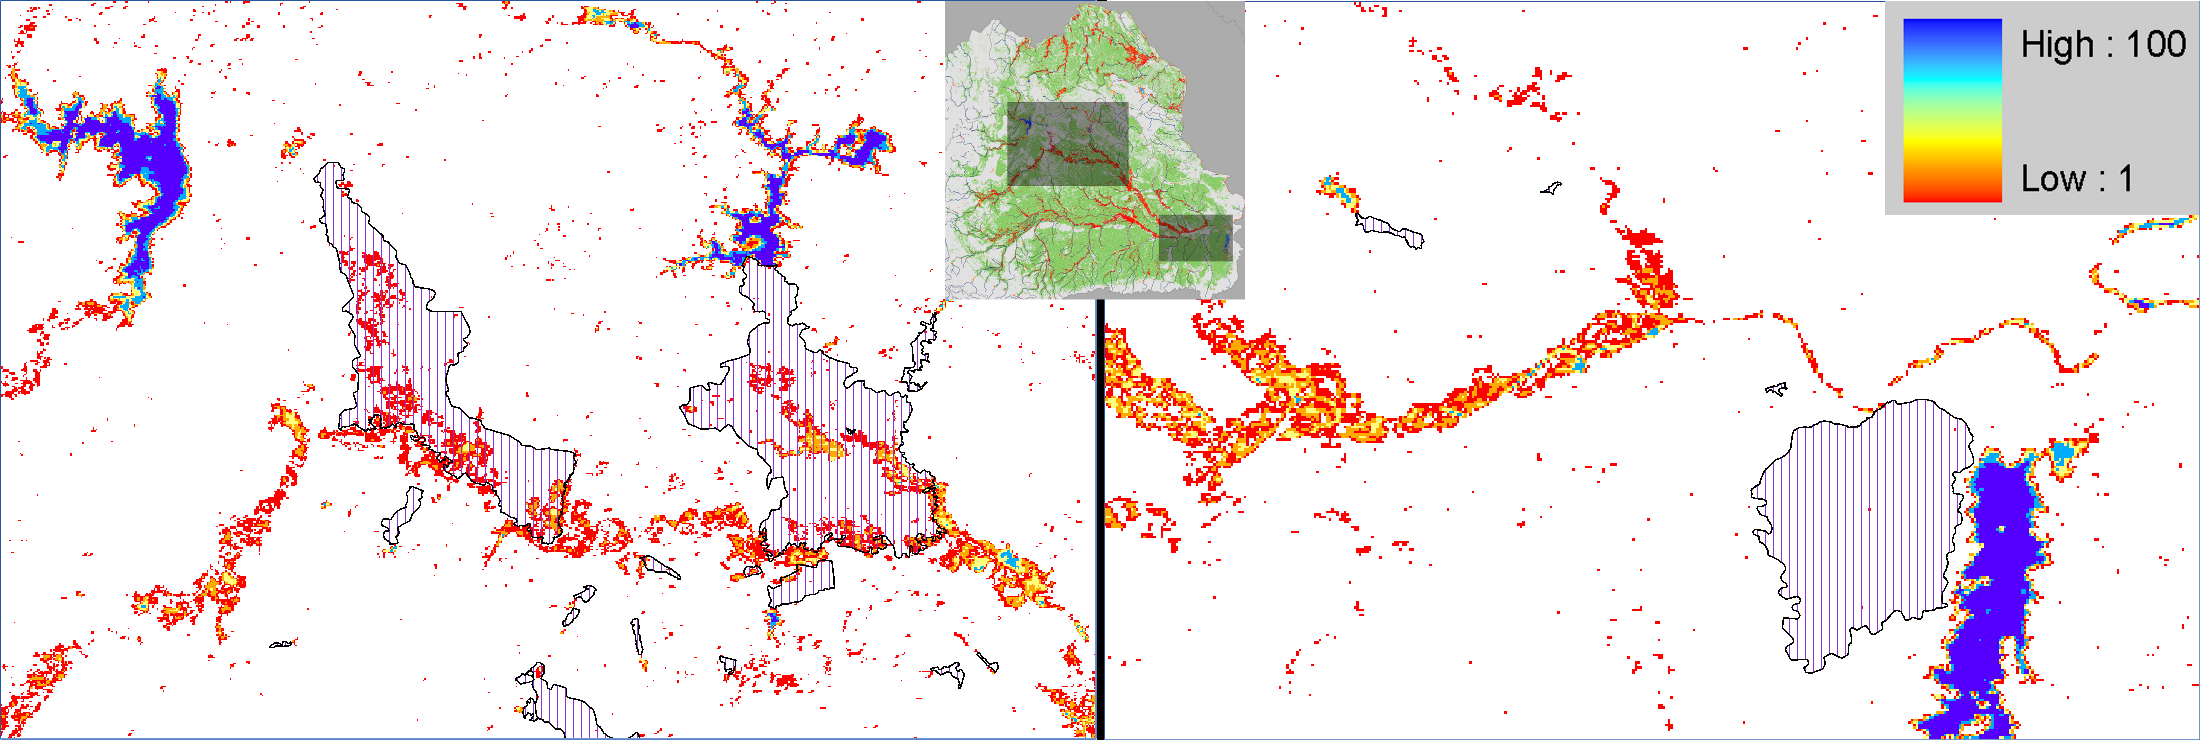
\includegraphics[width=11cm]{NETH_ASO_FREQ_irrig_area_insert_big_legend}\\
\end{tabular}
\end{flushleft}

\end{frame}


\section{Pakistan}
%%%%%%%%%%%%%%%%%%%%%%%%%%%%%%%%%%%%%%%%%%%%%%%%%%%%%%%%%%%%%%%%%%%%
\begin{frame}[fragile]{About Pakistan users...}

From a FOSS GIS user:
\begin{itemize}
 \item {\it Currently most the industry / NGOs are using pirated software}
 \item {\it When a project requires them to purchase a license, they opt for OSS and try to adopt it}
\end{itemize}

 \begin{itemize}
  \item The companies are not aware that OSS would require customisation and they have to pay for it
  \item Most of the NGOs opt for OSS
  \item In unis [..] perception that you have to be a geek to work on OSS as they would require a lot of programming
 \end{itemize}

\end{frame}

%%%%%%%%%%%%%%%%%%%%%%%%%%%%%%%%%%%%%%%%%%%%%%%%%%%%%%%%%%%%%%%%%%%%
\begin{frame}[fragile]{Solutions in Pakistan's context}

{\it Pakistan is a very suitable market because of low / no budget to purchase software licenses}

\begin{block}{{\it Solutions}}
\begin{itemize}
 \item {\it To educate the govt and ngo sector to opt for OSS from day one of the project cycle}
 \item {\it To make the training centers / universities offer OSS based trainings}
\end{itemize}
\end{block}

\end{frame}

\section{Sri Lanka}
%%%%%%%%%%%%%%%%%%%%%%%%%%%%%%%%%%%%%%%%%%%%%%%%%%%%%%%%%%%%%%%%%%%%
\begin{frame}[fragile]{About Sri Lanka's users...}

\begin{block}{{\it FOSSGIS appears in:}}
\begin{itemize}
 \item {\it Universities use FOSSGIS as a bargain chip to get ArcGIS licenses cheap/free}
 \item {\it }
\end{itemize}
\end{block}


\begin{block}{{\it Solutions}}
\begin{itemize}
 \item {\it Specific replacements (i.segment: huge uptake !)}
 \item {\it Spreading the word... ``We did not know it existed''}
\end{itemize}
\end{block}

\end{frame}


%%%%%%%%%%%%%%%%%%%%%%%%%%%%%%%%%%%%%%%%%%%%%%%%%%%%%%%%%%%%%%%%%%%%
\begin{frame}[fragile]{Colombo MC (from a student 20130707)}

\begin{center}
\begin{tabular}{l}
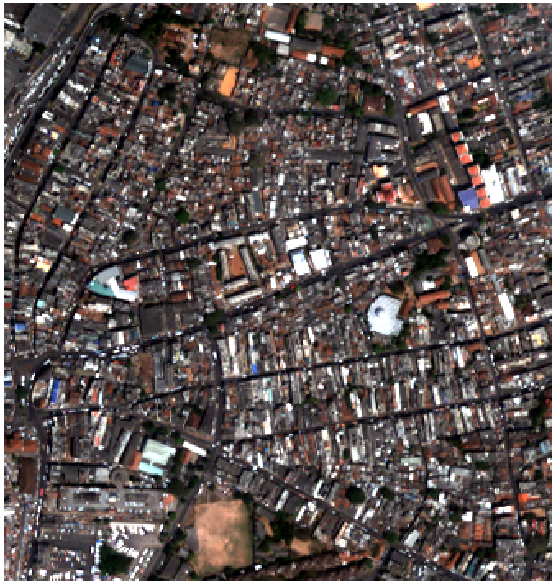
\includegraphics[width=5.5cm]{Qbird_orig}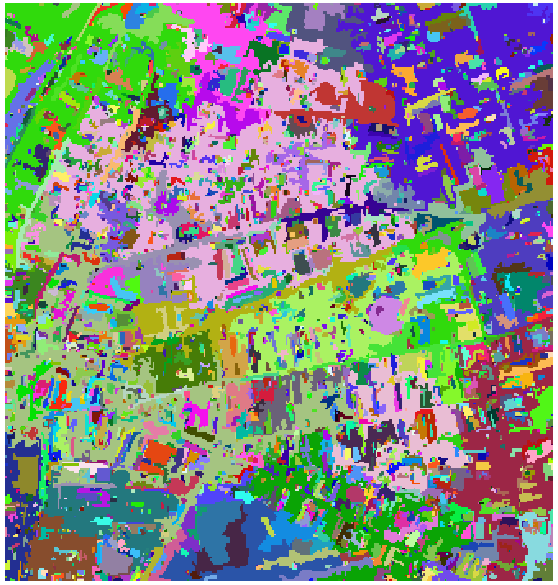
\includegraphics[width=5.5cm]{Qbird_seg}
\end{tabular}
First try, aiming to get road extracted from Quick Bird
\end{center}

\end{frame}


%%%%%%%%%%%%%%%%%%%%%%%%%%%%%%%%%%%%%%%%%%%%%%%%%%%%%%%%%%%%%%%%%%%%
\begin{frame}[fragile]{Sri Lanka Water Depletion by FOSSGIS}

\begin{center}
\begin{tabular}{l}
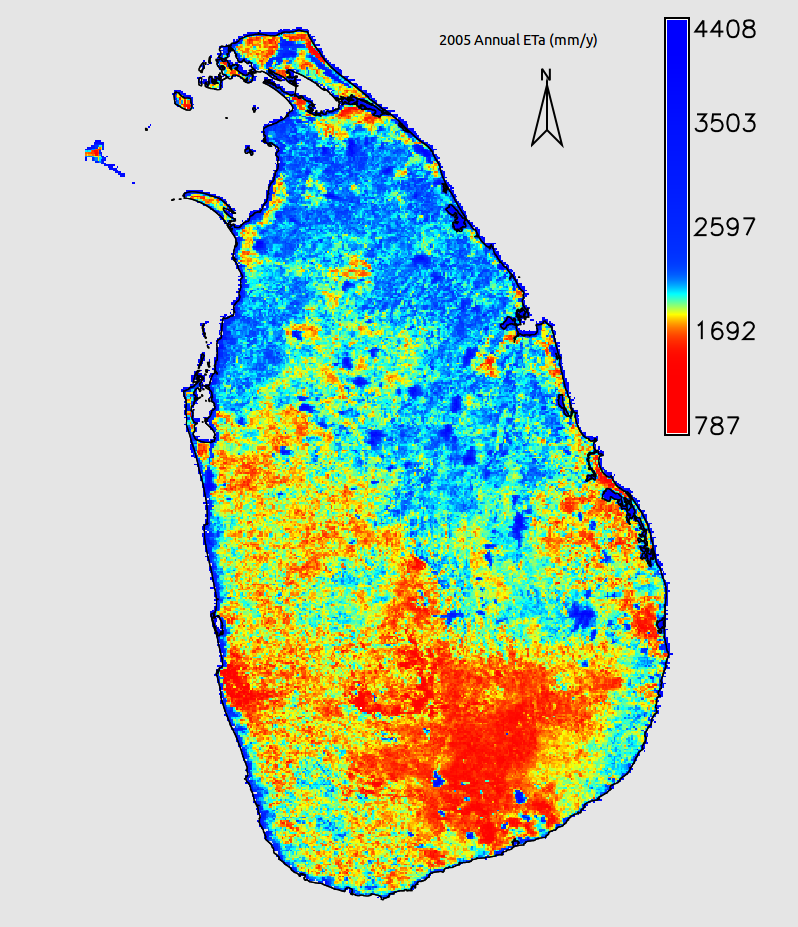
\includegraphics[width=5.5cm]{slet2005}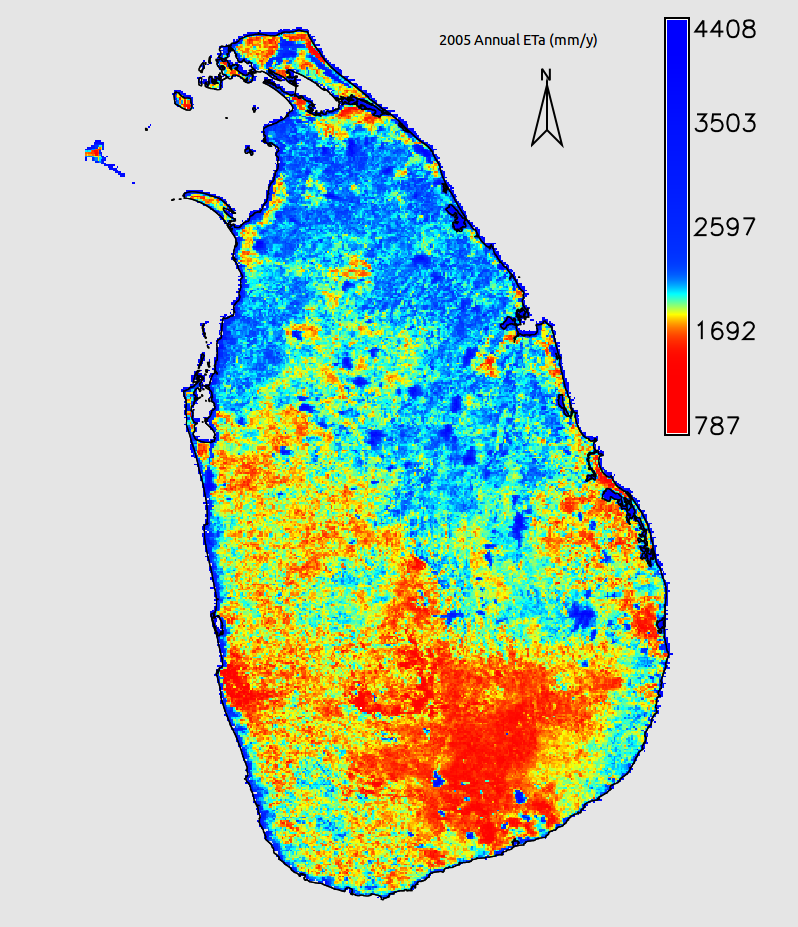
\includegraphics[width=5.5cm]{slet2005}
\end{tabular}
\end{center}

\end{frame}


\section{Not good yet}
%%%%%%%%%%%%%%%%%%%%%%%%%%%%%%%%%%%%%%%%%%%%%%%%%%%%%%%%%%%%%%%%%%%%
\begin{frame}[fragile]{The ``Not good yet'' syndrome}
A psychological hurdle seems not to be the ``no-cost=not good''
\begin{block}{from a non-FOSSGIS user in Thailand}
\begin{itemize}
\item {\it We used to have QGIS} \\
\item {\it But it produces not good results as ARCGIS} \\
\item Y: When was last time you used QGIS? \\
\item {\it Last 2 yrs}
\end{itemize}
\end{block}

\begin{block}{{\it But hope is there:}}
\begin{itemize}
\item Y: hmm, things have changed
\item {\it Better now?}
\item {\it I need to check it}
\item {\it Leave me a link to dl FOSSGIS or {\bf some works using it}}
\end{itemize}
\end{block}

\end{frame}

\section{Teaching}
%%%%%%%%%%%%%%%%%%%%%%%%%%%%%%%%%%%%%%%%%%%%%%%%%%%%%%%%%%%%%%%%%%%%
\begin{frame}[fragile]{In Universities}

There are adoptions in universities, essentially in research fields, BUT
\begin{block}{Reality check samples}
\begin{itemize}
 \item Freshmen computer literacy (Sri Lanka, Laos? etc.)
 \item Laos and Cambodia are Internet poor (Sri Lanka less) ... 
 \item Misconceptions about GIS (just make a map)
 \item GIS is essentially used to generate data in SSEA...
 \item No data openness (The Gollum Syndrome) from govt
\end{itemize}
\end{block}

\end{frame}

%%%%%%%%%%%%%%%%%%%%%%%%%%%%%%%%%%%%%%%%%%%%%%%%%%%%%%%%%%%%%%%%%%%%
\begin{frame}[fragile]{Universities to the help}

\begin{block}{Is it all a question of education?}
\begin{itemize}
 \item Large demand of technically proficient graduates
 \item Teaching faculty formatted to {\it standard} theoretical teaching
 \item Students rules of engagement low towards the faculty
 \item Memorizing concepts \& patterns, less experience driven
 \item Employability: first experience, challenge in some countries
\end{itemize}
\end{block}

\end{frame}

\section{Conclusions}
%%%%%%%%%%%%%%%%%%%%%%%%%%%%%%%%%%%%%%%%%%%%%%%%%%%%%%%%%%%%%%%%%%%%
\begin{frame}[fragile]{Conclusions}

\begin{enumerate}
 \item Change the mindset ``not good yet'' to positive experience?
 \item Can we spread the word on niche applications as entry points?
 \item Can we spend more time with students to empower them?
 \item FOSSGIS run in the mapping or the GIS Science arena?
 \item Asia has a large amount of people willing to try FOSSGIS... 
 \item How to help them to have the best first experience?
\end{enumerate}

\end{frame}

%%%%%%%%%%%%%%%%%%%%%%%%%%%%%%%%%%%%%%%%%%%%%%%%%%%%%%%%%%%%%%%%%%%%
\begin{frame}[fragile]{Thank You}

\ \\
\ \\
\ \\
\ \\
\ \\
\ \\
\ 
\begin{center}
\begin{tabular}{ll}

\includegraphics[width=3cm]{iwmi} & 
\includegraphics[width=2.6cm]{mrt}\\
\end{tabular}
\end{center}

\end{frame}

\end{document}
